%% Based on a TeXnicCenter-Template by Gyorgy SZEIDL.
%%%%%%%%%%%%%%%%%%%%%%%%%%%%%%%%%%%%%%%%%%%%%%%%%%%%%%%%%%%%%

%------------------------------------------------------------
%
\documentclass[titlepage]{article}%
%Options -- Point size:  10pt (default), 11pt, 12pt
%        -- Paper size:  letterpaper (default), a4paper, a5paper, b5paper
%                        legalpaper, executivepaper
%        -- Orientation  (portrait is the default)
%                        landscape
%        -- Print size:  oneside (default), twoside
%        -- Quality      final(default), draft
%        -- Title page   notitlepage, titlepage(default)
%        -- Columns      onecolumn(default), twocolumn
%        -- Equation numbering (equation numbers on the right is the default)
%                        leqno
%        -- Displayed equations (centered is the default)
%                        fleqn (equations start at the same distance from the right side)
%        -- Open bibliography style (closed is the default)
%                        openbib
% For instance the command
%           \documentclass[a4paper,12pt,leqno]{article}
% ensures that the paper size is a4, the fonts are typeset at the size 12p
% and the equation numbers are on the left side
%
\usepackage{amsmath}%
\usepackage{amsfonts}%
\usepackage{amssymb}%
\usepackage{graphicx}
\usepackage{listings}
\usepackage{color}

%-------------------------------------------
\renewcommand\abstractname{Summary}
\newtheorem{theorem}{Theorem}
\newtheorem{acknowledgement}[theorem]{Acknowledgement}
\newtheorem{algorithm}[theorem]{Algorithm}
\newtheorem{axiom}[theorem]{Axiom}
\newtheorem{case}[theorem]{Case}
\newtheorem{claim}[theorem]{Claim}
\newtheorem{conclusion}[theorem]{Conclusion}
\newtheorem{condition}[theorem]{Condition}
\newtheorem{conjecture}[theorem]{Conjecture}
\newtheorem{corollary}[theorem]{Corollary}
\newtheorem{criterion}[theorem]{Criterion}
\newtheorem{definition}[theorem]{Definition}
\newtheorem{example}[theorem]{Example}
\newtheorem{exercise}[theorem]{Exercise}
\newtheorem{lemma}[theorem]{Lemma}
\newtheorem{notation}[theorem]{Notation}
\newtheorem{problem}[theorem]{Problem}
\newtheorem{proposition}[theorem]{Proposition}
\newtheorem{remark}[theorem]{Remark}
\newtheorem{solution}[theorem]{Solution}
\newtheorem{summary}[theorem]{Summary}
\newenvironment{proof}[1][Proof]{\textbf{#1.} }{\ \rule{0.5em}{0.5em}}


% -------------------------------------------------
\newcommand{\oven}{\texttt{Oven}~}
\newcommand{\pgen}{\texttt{Paste Generator}~}
\newcommand{\paste}{\texttt{Paste}~}
\newcommand{\init}{\texttt{Initialization}~}
\newcommand{\ta}{\texttt{Time Advance}~}
\newcommand{\intt}{\texttt{Internal Transition}~}
\newcommand{\extt}{\texttt{External Transition}~}
\newcommand{\out}{\texttt{Output}~}
\newcommand{\bread}{\texttt{Bread}~}
\newcommand{\pd}{\texttt{PowerDEVS}~}

%For source code highliting
\definecolor{mygreen}{rgb}{0,0.6,0}
\definecolor{mygray}{rgb}{0.5,0.5,0.5}
\definecolor{mymauve}{rgb}{0.58,0,0.82}
\definecolor{mylgray}{rgb}{0.95,0.95,0.95}

\lstset{ %
  backgroundcolor=\color{mylgray},   % choose the background color
  basicstyle=\footnotesize,        % size of fonts used for the code
  breaklines=true,                 % automatic line breaking only at whitespace
  captionpos=b,                    % sets the caption-position to bottom
  commentstyle=\color{mygreen},    % comment style
  escapeinside={\%*}{*)},          % if you want to add LaTeX within your code
  keywordstyle=\color{blue},       % keyword style
  stringstyle=\color{mymauve},     % string literal style
	numbers=left,
	language=C++,
	basicstyle=\footnotesize\ttfamily
}

% --------------------------------------------------

\begin{document}

%======================================== Title Page ==================================
\pagestyle{empty}
\begin{center}

\includegraphics[scale=0.3]{TU-Signet.png}
\vspace{2cm}
{\huge \\Production Chain in a Bakery - DEVS\\}
\vspace{1cm}
{\Large Semester Project\\Modeling and Simulation (2014W)\\}

\vspace{3cm}
{Submitted To:\\}
\vspace{0.3cm}
{Univ.-Lecturer\\}
{Franz Josef Preyser\\}
{Institut für Analysis und Scientific Computing\\}
{Faculty of Informatics\\}

\vspace{2cm}
{Submitted By:\\}
\vspace{0.3cm}
{Jawad Haider KAZMI (1328102), \\ Ishtiaq AHMAD (1229645) and \\ Ikram ULLAH (1329824) \\}						%===== Your Name here
\vspace{2cm}
March, 2015
\end{center}
%========================================Table of Contents=====================================

\newpage
\tableofcontents
\newpage

%========================================Abstract===============================================
\begin{abstract}

The task of this project is to implement an simple DEVS-Model of a baking-oven with a DEVS-able simulation. The implemented model is described as follows;

At a certain point in time, portion of a paste with the attributes mass m and (up to now accumulated) costs K arrives at the Oven. If the oven is currently in the waiting - state (i.e. process-phase p=0), then the paste attributes a stored in the oven state variables m and K and the process-phase p is incremented (i.e. p:=1). This is all done by the external transition function $$\delta_{ext}$$. If process phase p=1, the paste is baking for the duration $$T_1$$. That is, the next event to be triggered is an internal event, which happened exactly T1 after the previous external event, where the paste arrived. This internal event leads to the execution of  $$\delta_{int}$$, which adds the costs K2 that arose from the baking phase to the accumulated costs K and increments the process phase p to p=2. p=2 means unloading-phase. The duration of the unloading phase is T2. Therefore after T2 the next internal event is triggered which again results in the execution of $$\delta_{int}$$. But this time , there is an output to be generated as well. So right before $$\delta_{int}$$ is executed, the output function lambda computed an "output-message". In our case, the output represents the baked bread, which again has the attributes mass m and costs K. the mass stays the same, so m will be set to the value stored as state variable m. Since the unloading phase also produce costs, the costs K will be set to the value stored as state variable K plus the costs K2 that arose in phase 2. After the output has been calculated, the internal transition function sets the state variables m and K to 0 also resets the process phase p to 0, meaning "waiting for the next paste to arrive." 
\vspace{1cm}

%\noindent {\large \bfseries{Keywords:~}} 
\end{abstract}


%======================================== Main Text =====================================
\newpage
\setcounter{page}{1}
\pagestyle{plain}

\section{Task-1 DEVS-Model  for Baking Oven}

\subsection{Description}

The task of this project is to implement an simple DEVS-Model of a baking-oven with a DEVS-able simulation. The implemented model is described as follows;
At a certain point in time, portion of a paste with the attributes mass m and (up to now accumulated) costs K arrives at the Oven. If the oven is currently in the waiting - state (i.e. process-phase p=0), then the paste attributes a stored in the oven state variables m and K and the process-phase p is incremented (i.e. p:=1). This is all done by the external transition function $$\delta_{ext}$$ . If process phase p=1, the paste is baking for the duration T1. That is, the next event to be triggered is an internal event, which happened exactly T1 after the previous external event, where the paste arrived. This internal event leads to the execution of  $$\delta_{int}$$ , which adds the costs K2 that arose from the baking phase to the accumulated costs K and increments the process phase p to p=2. p=2 means unloading-phase. The duration of the unloading phase is T2. Therefore after T2 the next internal event is triggered which again results in the execution of $$\delta_{int}$$. But this time , there is an output to be generated as well. So right before $$\delta_{int}$$ is executed, the output function lambda computed an "output-message". In our case, the output represents the baked bread, which again has the attributes mass m and costs K. the mass stays the same, so m will be set to the value stored as state variable m. Since the unloading phase also produce costs, the costs K will be set to the value stored as state variable K plus the costs K2 that arose in phase 2. After the output has been calculated, the internal transition function sets the state variables m and K to 0 also resets the process phase p to 0, meaning "waiting for the next paste to arrive." 

\subsection{Paste arrive scenario}
We have implemented a \texttt{Queue} to handle the situation when the process phase p is not zero and a paste arrives. If p is not zero and a paste is ready , it is added to the queue. After the execution of internal function and completion of phase 2 , queue is checked , if it is not empty then paste is picked from the queue on the basis of first in first out (FIFO). 

\section{Task-2 : Implementation of Baking Oven Model in \pd}

The DEVS model of the Baking Oven is shown in Fig. \ref{fig:model}. The models shows that the 
implementation consists of four atomic models (\pgen, \oven, 
{\ttfamily{Plot}} and {\ttfamily{Save to Disk}}), two (\pgen and 
{\oven) of which are programmed by us while the other two ({\ttfamily{Plot}} and 
{\ttfamily{Save to Disk}}) are used from the PowerDEVS's library. The \pgen 
generates random \paste with mass and processing times. The \paste 
is then processed (baked) in the \oven and a \bread is produced. 

\begin{figure}[htbp]
	\centering
		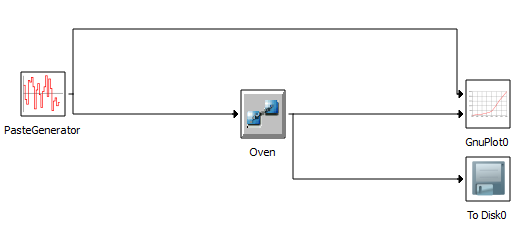
\includegraphics[scale=0.8]{model.PNG}
	\caption{The Baking Oven Model in PowerDEVS}
	\label{fig:model}
\end{figure}

\subsection{Paste structure}

A structure is created to hold the parameters and to describe the paste. The definition of the structure is shown in the Listing \ref{paste}.

\begin{lstlisting}[caption={Paste structure}, language=c++, label={paste}]

struct Paste
{
    double mass;         // Mass of the paste
    double p1Time;       // Baking time required in P1
    double p2Time;       // Baking time required in P2
    double bakingCost;   // Baking cost
	
    double tArrival;     // Arrival time
    double tDeparture;   // Departure time (when baked as bread)
};

\end{lstlisting}


\subsection{Paste Generator}
The {\ttfamily{Paste Generator}} can be configures to produce randomly varying the values according to the configured parameters. In PowerDEVS IDE, the parameters dialog box is for {\ttfamily{Paste Generator}} is shown in the Fig. \ref{fig:pastegen_params}.

\begin{figure}[htbp]
	\centering
		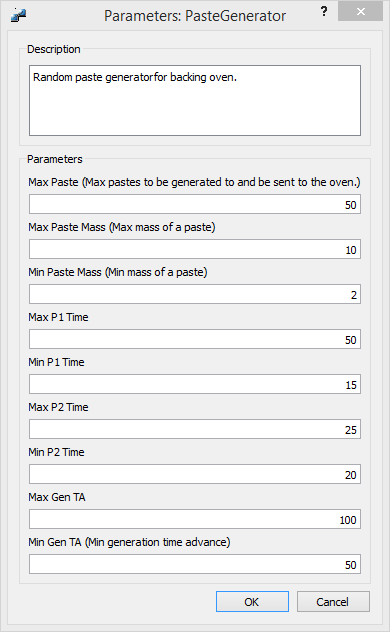
\includegraphics[scale=0.8]{pastegen_params.PNG}
	\caption{{\ttfamily{Paste Generator}} parameters configuration dialog-box in PowerDEVS IDE}
	\label{fig:pastegen_params}
\end{figure}

Listing \ref{pg_state_var} below, shows the state variables and objects used during the paste generation.

\begin{lstlisting}[caption={State variables and objects}, language=c++, label={pg_state_var}]

  double sigma;            // The TA value

  StochasticLib1 *stor;    // Lib for RN Generation
  Paste* paste;            // The paste structure object

  //Parameters
  double maxOutputs;       // Max pastes to be generated
  double massMax, massMin; // Mass
  double p1Max, p1Min;     // P1 time 
  double p2Max, p2Min;     // P2 time
  double genMax, genMin;   // Generation pause

\end{lstlisting}

Listing \ref{pg_init} is the \init routine for the Paste Generator. The line 1,2 is the call for passing the parameters from the IDE to a list. This list is later used to assign the configured values to the state variable (line 5--13). Next,  StochasticLib1 \footnote{http://gull.sourceforge.net/dev/classStochasticLib1.html} is initialized with a seed generated from the timer and a random number (15--16). The TA value state variable sigma is initialized to 0 (line 18). At the end, a a summary of the configured parameters is printed into the log file (lines 21--27).

\begin{lstlisting}[caption={The \init for the \pgen }, language=c++, label={pg_init}]
va_list parameters;
va_start(parameters,t);

maxOutputs=va_arg(parameters,double);	//Max pastes

massMax=va_arg(parameters,double); //Max mass
massMin=va_arg(parameters,double); //Min mass
p1Max=va_arg(parameters,double);  //Max p1 time
p1Min=va_arg(parameters,double); //Min p1 time
p2Max=va_arg(parameters,double); //Max p2 time
p2Min=va_arg(parameters,double); //Min p2 time
genMax=va_arg(parameters,double); //Max ta for output
genMin=va_arg(parameters,double); //Min ta for output

int seed = (int)time(0)+rand(); //seed for random num lib
stor=new StochasticLib1(seed); //Initialized the lib

sigma=0;												

//Print summary of the configured parameters
printLog("Paste Generator configured with:\n");
printLog("\tMax Pastes=%g\n", maxOutputs);
printLog("\tMax Mass=%g, Min Mass=%g\n", massMax, massMin);
printLog("\tMax P1=%g,   Min P1=%g\n", p1Max, p1Min);
printLog("\tMax P2=%g,   Min P2=%g\n", p2Max, p2Min);
printLog("\tMax Gen TA=%g,   Min Gen TA=%g\n", genMax, genMin);
printLog("\t----------------------------\n\n\n");
\end{lstlisting}	


The time advance (TA) routine (Listing \ref{pg_ta}), generates and returns a random double value between \texttt{genMin} and \texttt{genMax} state variable untill the configured numbers of pastes (\texttt{maxOutputs}) have been generate. Otherwise it returns the maximum allowed values for a variable of type double (\texttt{std::numeric\_limits<double>::max()}).

\begin{lstlisting}[caption={The TA (Time Advance) function}, language=c++, label={pg_ta}]
//Time Advance (TA)

//Check if the configured number of
//outputs have been generated.
if(maxOutputs>0) {
  return sigma;
}
else {
  return std::numeric_limits<double>::max();
}
\end{lstlisting}	

The Internal Transition function (Listing \ref{pg_it}) simply generates a random value between the configured parameter \texttt{genMin} and \texttt{genMax} and assigned to a state values, for next time advance.

\begin{lstlisting}[caption={The Internal Transition function for the \pgen}, language=c++, label={pg_it}]
//The Internal Transition
sigma=stor->IRandom(genMin,genMax);
\end{lstlisting}

Since, \pgen has no input interface, so it has nothing in the External Transition routine.

The Output function is show in the Listing \ref{pg:ot}. A \paste is first created and than, its parameters are filled with random values under the configured range and then sent to the output port. Once, enough \paste have been generated than an \texttt{empty} output is returned.
 
\begin{lstlisting}[caption={The Output function for the \pgen}, language=c++, label={pg:ot}]
if(maxOutputs-->0)
{
 paste=new Paste();
 paste->mass=stor->IRandom(massMin,massMax);
 paste->p1Time=stor->IRandom(p1Min,p1Max);
 paste->p2Time=stor->IRandom(p2Min,p2Max);

 // Record in the Even Log
 printLog("[PASTEGEN] Generated paste number \%d with mass=\%g, p1Time=\%g, p2Time=\%g\n",
	maxOutputs, paste->mass, paste->p1Time, paste->p2Time);

 return Event(paste, 0);
}
else return Event();

\end{lstlisting}


\subsection{Oven}
The \oven is modeled as a bakery oven having two baking stages. Each stage has an associated per time unit cost that can be configured in PowerDEVS using the parameters configuration dialog-box shown in the Figure \ref{fig:oven_params}.
\begin{figure}[htbp]
	\centering
		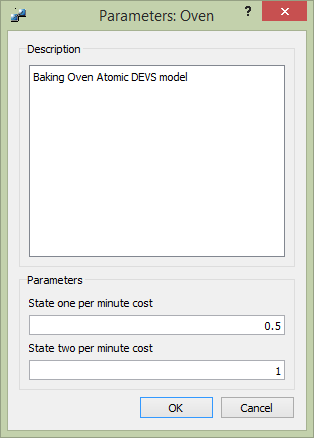
\includegraphics[scale=0.8]{oven_params.PNG}
	\caption{{\ttfamily{Oven}} configuration parameters dialog-box in PowerDEVS IDE}
	\label{fig:oven_params}
\end{figure}

Listing \ref{o_state_var}, below shows the state variables and objects used by the \oven.

\begin{lstlisting}[caption={State variables and objects used by \oven}, language=c++, label={o_state_var}]
// Clock
double clock;

//List of waiting pastes
std::list <Paste*> pasteQueue;

Paste* bread;

//Current oven state (0, 1, 2)
int processState;

int processed;

double p1Cost, p2Cost, totalCost;
double waitingTime;
int sendOutput;

\end{lstlisting}

The code for the \init function of \oven is shown in Listing \ref{o_init}.

\begin{lstlisting}[caption={\init function for \oven}, language=c++, label={o_init}]
va_list parameters;
va_start(parameters,t);

p1Cost=va_arg(parameters,double);
p2Cost=va_arg(parameters,double);

clock=0;			// Reset the clock
tUtilized=0;		// Reset

processState=0;
totalCost=0;
sendOutput=0;
processed=0;
waitingTime=0.0;


printLog("Oven Initilized clock=\%g, state=\%d\n", clock, processState, t);
printLog("\tConfigured with p1Cost=\%g, p2Cost=\%g\n================================================\n\n", p1Cost, p2Cost);

\end{lstlisting}
\begin{lstlisting}[caption={\ta function for \oven}, language=c++, label={o_ta}]
double sigma;

switch(processState){
	case 0:		// We should never arrive here!
		if(pasteQueue.empty()){
			printLog("[OVEN]->[TA] No paste to bake, waiting for the paste INF (state=\%d)\n", processState);		
			sigma=std::numeric_limits<double>::max();
		}
		else sigma=pasteQueue.front()->p1Time;
		break;
	case 1:		// processState1
		sigma=pasteQueue.front()->p1Time;
		break;
	case 2:		// processState2
		sigma=pasteQueue.front()->p2Time;
		break;
	default:	// an invalid state
		sigma=std::numeric_limits<double>::max();
}

//sigma+=clock;
if(!t==0) printLog("[OVEN]->[TA] clock=\%g, state=\%d, sigma=\%g\n", clock, processState,sigma);

return sigma;
\end{lstlisting}

\begin{lstlisting}[caption={\intt function for \oven}, language=c++, label={o_ta}]
int dummy;

clock+=ta(0);		//Update clock

switch(processState){
	case 0:
		if(!pasteQueue.empty()) dummy=1;
		else dummy=0;
	case 1:
		dummy=2;
		break;
	case 2:
		sendOutput=1;	
		bread = pasteQueue.front();			
		//beingBakedPaste=pasteQueue.front();
		if(pasteQueue.empty()) { dummy=0; }
		else {
			dummy=1;			
		}
		pasteQueue.pop_front();
		break;	
}
processState=dummy;

printLog("[OVEN]->[INT] clock=\%g, New state=\%d\n", clock, processState);
\end{lstlisting}

\begin{lstlisting}[caption={\extt function for \oven}, language=c++, label={o_ext}]
// update the clock
clock += e;

if(processState==0){
	processState=1;	
}

pasteQueue.push_back((Paste*)x.value);
pasteQueue.back()-> tArrival = clock;

//beingBakedPaste = 
printLog("[OVEN]->[EXT] at clock=\%g, New paste addedd.\n", clock);
printLog("\t[EXT] Queue lenght is \%d.\n", pasteQueue.size());
\end{lstlisting}


\begin{lstlisting}[caption={\out function for \oven}, language=c++, label={o_output}]
if(sendOutput==1){

	sendOutput=0;
	processed++;

	//Paste* bread = pasteQueue.front();

	bread->tDeparture=clock;
	bread->bakingCost = (bread->p1Time * p1Cost) + (bread->p2Time * p2Cost);
	totalCost += bread->bakingCost;
	waitingTime += bread->tDeparture-bread->tArrival;

	printLog("[OVEN]->[OUTPUT] clock=\%g, Mass=\%g, p1Time=\%g, p2Time=\%g, Cost=\%g, Accumulated Cost=\%g, tArrival=\%g, tDepart=\%g, tWait=\%g\n", 
			clock, bread->mass, bread->p1Time, bread->p2Time, bread->bakingCost,totalCost, bread->tArrival, 
			bread->tDeparture, bread->tDeparture-bread->tArrival);

	printLog("\t[OUTPUT] Queue lenght is \%d.\n", pasteQueue.size());	
	
	return Event(bread, 0);
}
else{
	return Event();
}
\end{lstlisting}

\begin{lstlisting}[caption={Exit function for \oven}, language=c++, label={o_exit}]
//Code executed at the end of the simulation.
printLog("==================OVEN===========================\n");
printLog("\tClock=\%g", clock);
printLog("\tAccumulate Cost = \%g\n", totalCost);
printLog("\tAverage Waiting Time = \%g\n", waitingTime/processed);
printLog("\tPastes Processed = \%d\n", processed);
printLog("=============================================\n");
\end{lstlisting}


\section{Task-3 : Documentation}
\subsection{DEVS-Formalism}

DEVS is an acronym for Discrete Event System . This is a formalism that was first introduced by Bernard Zeigler. It is used for the description of discrete event system.  A DEVS model has input events which are processed to produce output events(results). Output events are influenced by  input events and  initial conditions of the model.Figure \ref{atomic_model} shows a basic structure of an atomic model.  An Atomic DEVS model has the following formulation;

Where

$$X$$ 		: set of input event values, i.e., the set of all possible values that an input event can have \\
$$Y$$ 		: set of possible output event values \\
$$S$$ 		: set of possible states values \\
$$\delta ext$$ 	: External state transition function \\
$$\delta int$$ 	: Internal state transition function \\
ta	  	: Time advance  Function \\

\begin{figure}[ht!]
  \centering
    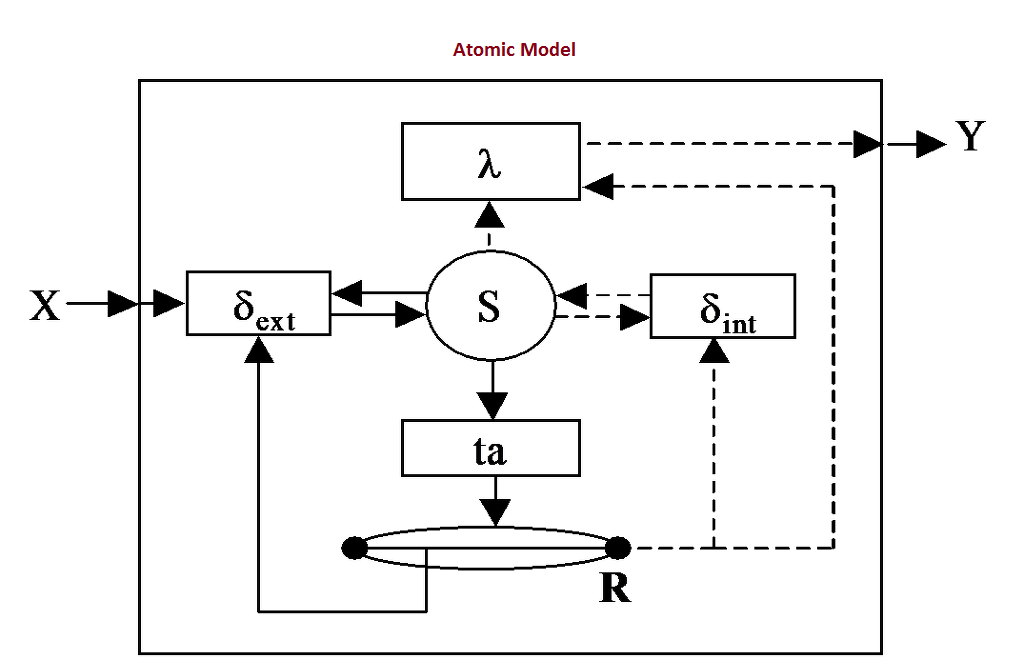
\includegraphics[width=0.5\textwidth]{Fig1.png}
    \caption{Atomic Model}
    \label{atomic_model}
\end{figure}


\subsection{DEVS-Model for Baking Oven}
\subsection{Simulation Tool Experiences}


PowerDEVS is a general purpose software tool for DEVS modeling and simulation oriented to the simulation of hybrid systems. It allows defining atomic DEVS models in C++ language that can be then graphically coupled in hierarchical block diagrams to create more complex systems. The environment automatically translates the graphically coupled models into a C++ code which executes the simulation \cite{BK11}.
One of the features of PowerDEVS is the synchronization of simulation in real time operating system with real time clock, which allows the design and implementation of synchronous and asynchronous digital controller. PowerDEVS is also efficient tool for real time simulation of physical systems when combined with continuous system simulation library. The interconnection of PowerDEVS with the numerical package Scilab is another attractive feature of PowerDEVS. The variables and functions in the workspace of Scilab can be used by PowerDEVS, and Scilab can process and analyze the result data sent from PowerDEVS.
PowerDEVS is composed of various independent programs: 



\subsubsection{The Model Editor} 
It is the main program of PowerDEVS which provides graphical interface for building and managing models and library, launching simulation, editing elementary blocks up to atomic model definitions and link with other application of PowerDEVS. 
 
 
 \begin{figure}[ht!]
  \centering
    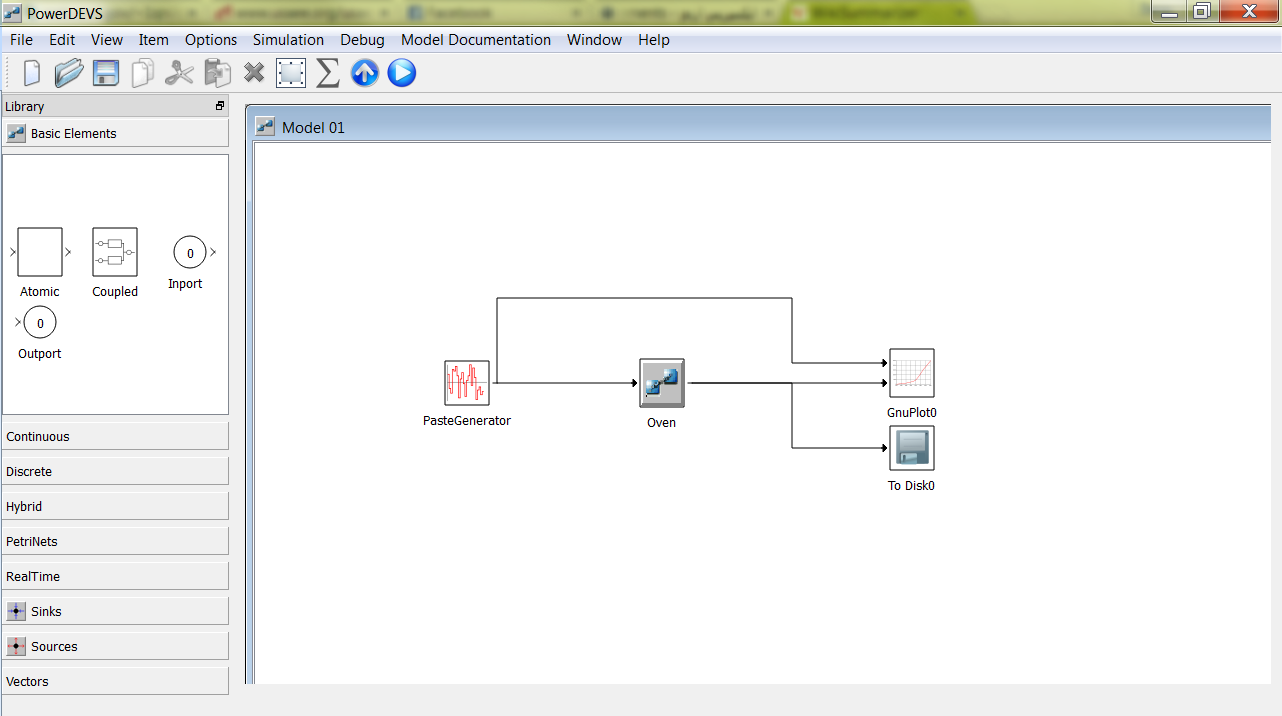
\includegraphics[width=0.5\textwidth]{Fig2.png}
    \caption{Model Editor main window}
    \label{model_edt}
\end{figure}
 
The Model Editor main window shown in Figure \ref{model_edt} is used to create and open models and libraries. At the left the list if libraries can be selected and blocks can be dragged from the libraries to the models. The selected library is active and the blocks are visible under the selected library. Models and libraries can be edited in a model window with the open and new model commands. The model window in Figure \ref{model_win} showing model consist of with four sub models.


 \begin{figure}[ht!]
  \centering
    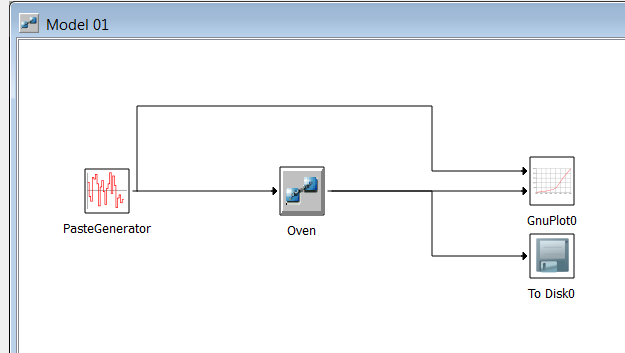
\includegraphics[width=0.5\textwidth]{Fig3.png}
    \caption{Model Window}
    \label{model_win}
\end{figure}

In the model windows the typical graphical edition facilities are provided so that blocks can be copied, resized, rotated, etc. while the connections between different ports can be directly drawn. The edit menu or using the right button the features of each blocks either a coupled or an atomic model can be edited. The block edition window shown in Figure \ref{Block_win} is used to configure the graphic appearance of the block and to choose the parameters of blocks. In the case of atomic models the associated code with the DEVS model definitions, can be selected in block edition window. The values of the block parameters can be changed by double clicking on the block as shown in Figure \ref{para_win} . Thus the predefined blocks are taken from the libraries and the parameter values can be changed without editing them.

\begin{figure}[ht!]
  \centering
    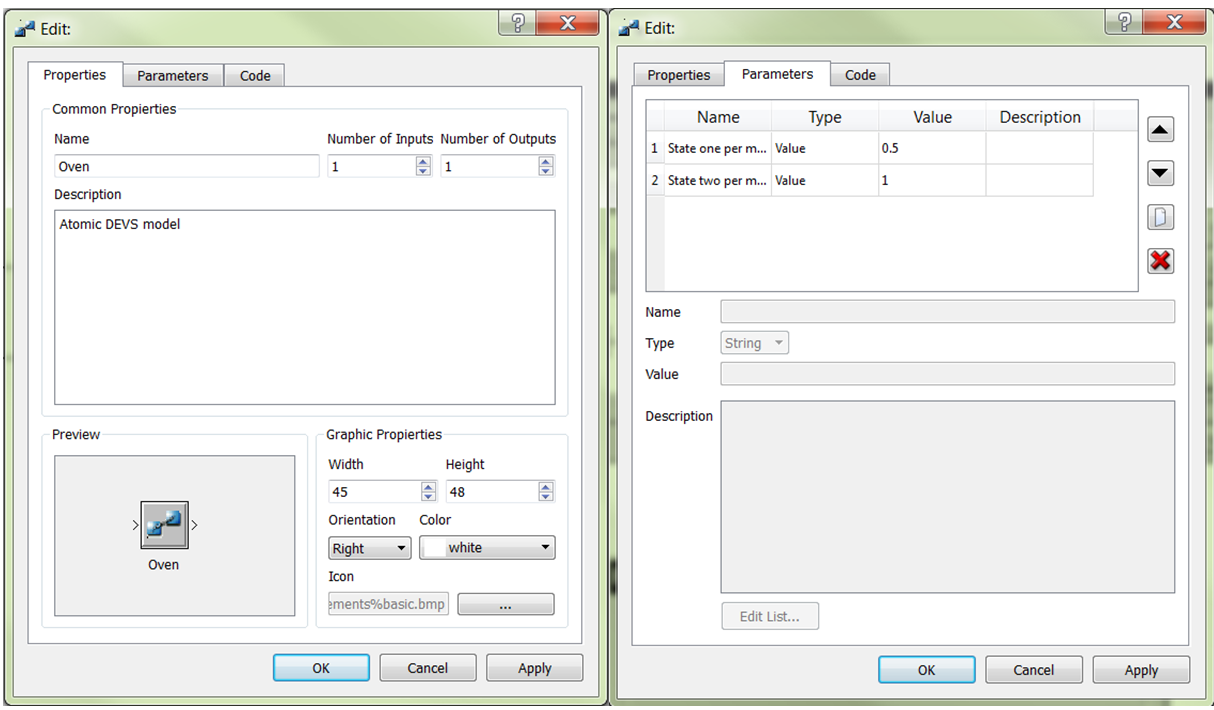
\includegraphics[width=0.85\textwidth]{Fig4.png}
    \caption{Block Edition Window}
    \label{Block_win}
\end{figure}

The Coupled models have no an associated code and there are some other extra features which can be modified in block edition window and the edit menu. Various input and output ports of a coupled model are characterized by their names. The order of their appearance in the block can be changed in the edition window. Priorities can be established in edition menu of corresponding model to solve the simultaneous occurrence of event among blocks at the same sub–model.

\begin{figure}[ht!]
  \centering
    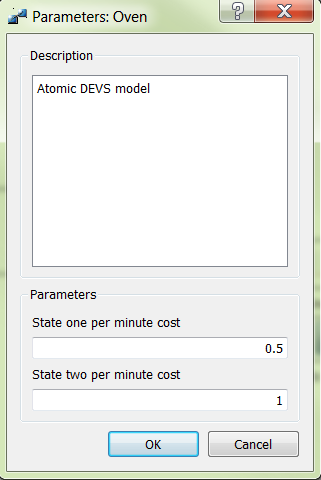
\includegraphics[width=0.5\textwidth]{Fig5.png}
    \caption{Parameter changing window}
    \label{para_win}
\end{figure}


\subsubsection{The Atomic Editor}
The Atomic Editor facilitates the edition of C++ code corresponding to each DEVS model. The transition functions, output function, time advance, etc. for DEVS atomic models of elementary blocks are defined in it.


\begin{figure}[ht!]
  \centering
    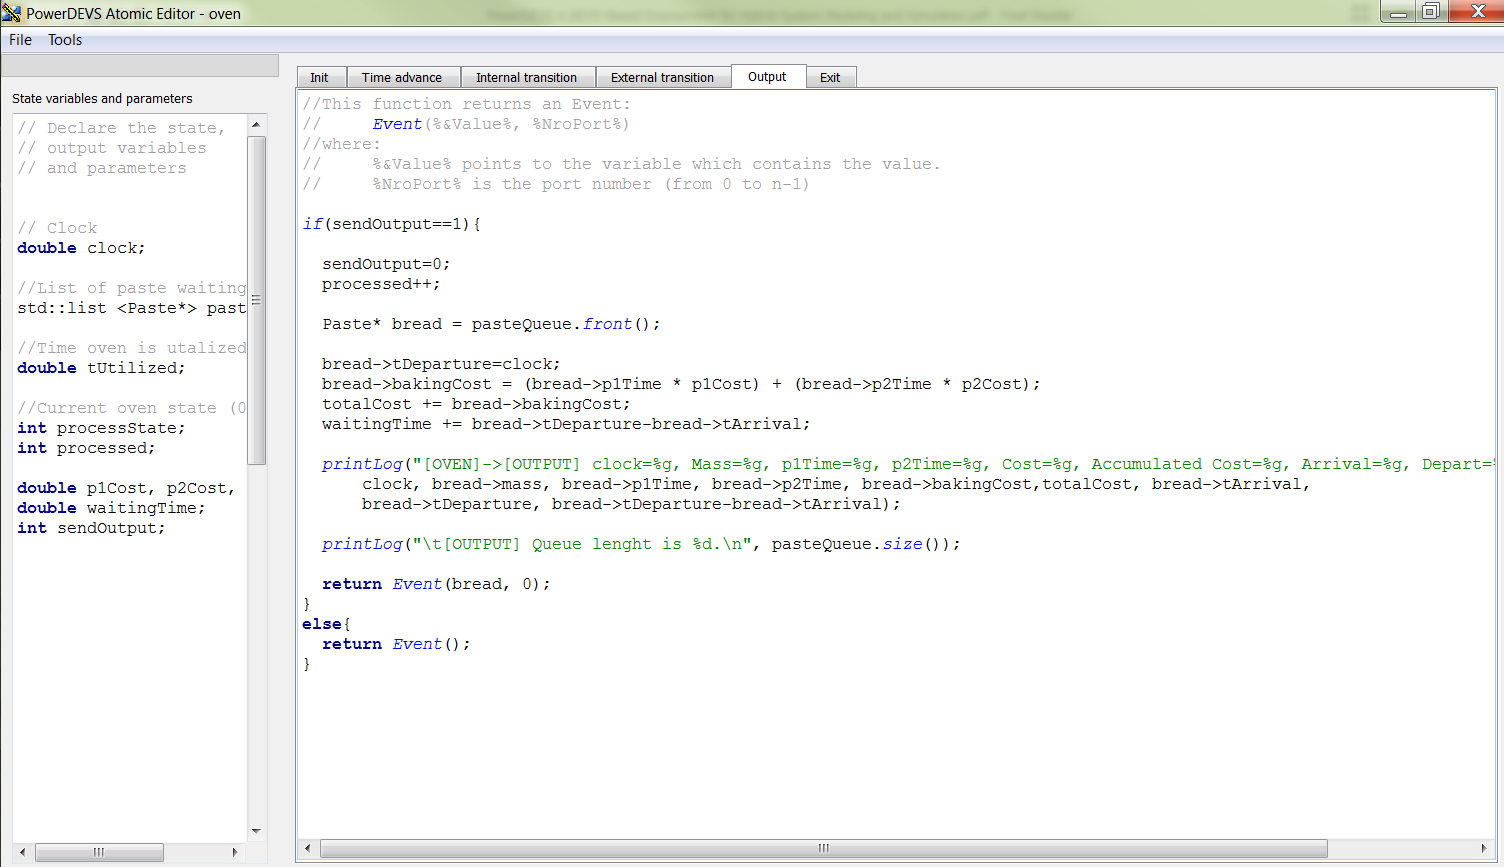
\includegraphics[width=0.9\textwidth]{Fig6.png}
    \caption{Atomic Editor main window}
    \label{atomic_win}
\end{figure}

It can be invoked from the Edition Window to edit an existing code or to create a new one. It can be also run directly from Windows since it is a standalone application. The Atomic Editor main window is shown in Figure \ref{atomic_win}. In atomic editor the state variables, the output of the DEVS model and the variables of system parameters are only defined. Then the C++ code for time advance, transition and output functions has to be placed in the corresponding windows and when the model is saved, the code is automatically completed and stored in the corresponding .cpp and .h files. The Atomic Editor was also designed to write a code which is very similar to the DEVS model definition. All the rest of the job related to simulation and implementation topics is automatically performed by the program.
\subsubsection{Structure Generator}
A PowerDEVS model is defined by block diagram in dot pdm file which represent system structure and the atomic models in dot h and dot cpp files which are generated by the atomic editor. Then, the simulation is run using Quick Simulation command in the Simulation menu of the Model Editor. The Quick Simulation command performs the simulation and PowerDEVS model is converted into a standalone program that executes the simulation. The final simulation time is only asked in this command and then the simulation is executed.
The conversion of the model into a simulation program is done in two steps. The Structure Generator converts the model file (.pdm) which contains all the information about the model, into a coupled DEVS specification. The Structure Generator produces a dot pds file which only contains the information about connections, location of atomic models and block parameters, etc., needed to build the simulation file. The coupling specification of the model is also converted into a formal DEVS coupling specification. As the Structure Generator is a standalone program so it can be run directly from the Simulation menu or from the command line. If it is run in that way, it produces a report in dot pds file showing the output. Figure \ref{Struc_gen} shows the out of structure generator.


\begin{figure}[ht!]
  \centering
    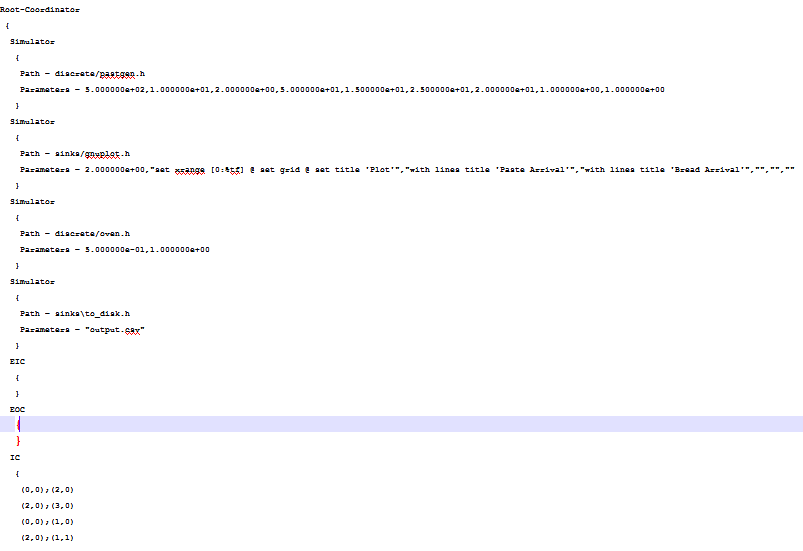
\includegraphics[width=0.9\textwidth]{Fig7.png}
    \caption{Structure Generator output}
    \label{Struc_gen}
\end{figure}



\subsubsection{The Preprocessor}
The Preprocessor translates the model editor files into structure files which contain the coupling structure and the information to build up the simulation code, links the code of the different atomic models according to the corresponding structure file and compiles it to produce a standalone executable file which simulates the system. It basically translates the .pds file into a header dot h file which binds the simulators and coordinators according to the coupling structure. The preprocessor also produces a make file which is then invoked to generate the program which executes the simulation. The Preprocessor can be invoked in a transparent way using the Quick Simulation command.
\subsubsection{The Simulation Interface }
The Simulation Interface ( Figure \ref{sim_int} ) runs the stand alone executable files according to the structure of PowerDEVS as shown in Figure \ref{sim_st} and provides to change the parameters of simulation like final time, number of simulations to perform, and the simulation mode (normal simulation, timed simulation, step-by-step simulation, etc.).


\begin{figure}[ht!]
  \centering
    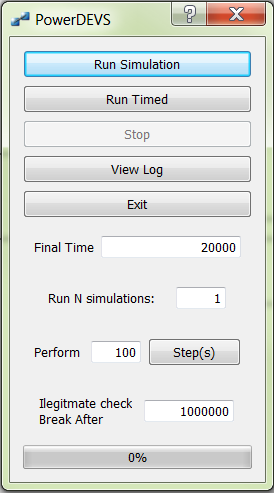
\includegraphics[width=0.5\textwidth]{Fig8.png}
    \caption{Simulation interface}
    \label{sim_int}
\end{figure}


\begin{figure}[h!]
  \centering
    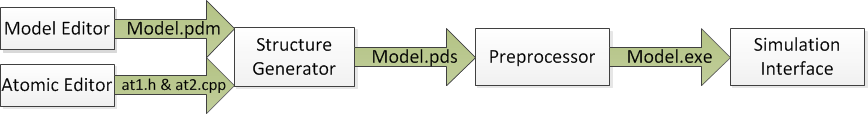
\includegraphics[width=0.7\textwidth]{Fig9.png}
    \caption{Simulation structure of PowerDEVS}
    \label{sim_st}
\end{figure}


 
\subsubsection{A running instance of Scilab}

It acts as a workspace, where the simulation parameters can be read and results can be exported to. This instance is a modification of Scilab 4.1.2 to support this type of operations as shown in Figure \ref{sci_in}.




\begin{figure}[ht!]
  \centering
    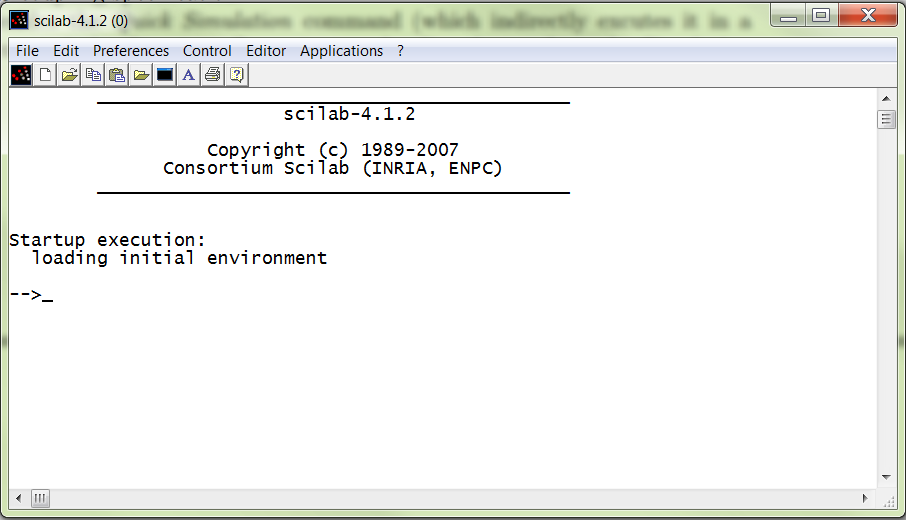
\includegraphics[width=0.7\textwidth]{Fig10.png}
    \caption{Scilab Instance}
    \label{sci_in}
\end{figure}

All the applications of PowerDEVS except Model Editor were programmed in C++ with the graphical libraries QT and Model Editor was only application programmed in Visual Basic. PowerDEVS can runs under a real time operating system (\cite{ManRTI}) synchronizing the event with a real–time clock with the capability of capturing interrupts at the atomic level. PowerDEVS also allows the direct implementation of asynchronous DEVS–based Quantized State Controllers \cite{Kof03b} on a PC.




%\subsection{Power DEVS implementation Details}
%\subsection{Most challenging subtask of the project}




\section{Task 4 : Simulation Results}

%\section{Results}

Log file listing
\begin{verbatim}
Paste Generator configured with:
	Max Pastes=2
	Max Mass=10, Min Mass=2
	Max P1=50,   Min P1=15
	Max P2=25,   Min P2=20
	Max Gen TA=100,   Min Gen TA=50
	----------------------------


Oven Initialized clock=0, state=0
	Configured with p1Cost=0.5, p2Cost=1
================================================

Simulation Initialized
[OVEN]->[TA] No paste to bake, waiting for the paste INF (state=0)
[PASTEGEN] Generated paste number 1 with mass=3, p1Time=35, p2Time=25
[OVEN]->[EXT] at clock=0, New paste addedd.
   [EXT] Queue length is 1.
[OVEN]->[INT] clock=35, New state=2
[OVEN]->[TA] clock=35, state=2, sigma=25
[OVEN]->[INT] clock=60, New state=1
[OVEN]->[TA] clock=60, state=1, sigma=35
[PASTEGEN] Generated paste number 0 with mass=2, p1Time=29, p2Time=23
[OVEN]->[EXT] at clock=79, New paste addedd.
   [EXT] Queue length is 1.
[OVEN]->[TA] clock=79, state=1, sigma=29
[OVEN]->[OUTPUT] clock=79, Mass=3, p1Time=35, p2Time=25, Cost=42.5, 
>>>>>>Accumulated Cost=42.5, tArrival=0, tDepart=79, tWait=79
   [OUTPUT] Queue length is 1.
[OVEN]->[INT] clock=108, New state=2
[OVEN]->[TA] clock=108, state=2, sigma=23
[OVEN]->[INT] clock=131, New state=1
[OVEN]->[TA] clock=131, state=1, sigma=29
[OVEN]->[OUTPUT] clock=131, Mass=2, p1Time=29, p2Time=23, Cost=37.5, 
>>>>>Accumulated Cost=80, tArrival=79, tDepart=131, tWait=52
   [OUTPUT] Queue length is 0.
[OVEN]->[INT] clock=160, New state=2
[OVEN]->[TA] clock=160, state=2, sigma=23
[OVEN]->[INT] clock=183, New state=0
[OVEN]->[TA] No paste to bake, waiting for the paste INF (state=0)
[OVEN]->[TA] clock=183, state=0, sigma=1.79769e+308
==================OVEN===========================
	Clock=183	Accumulate Cost = 80
	Average Waiting Time = 65.5
	Pastes Processed = 2
=============================================
Simulation Ended (0.008 sec)

(>>>>>> indicates a continued line with the previous)
\end{verbatim}


%========================================Bibliography=====================================
\bibliographystyle{plain}


\bibliography{ref}

%========================================Appendix=====================================

%\newpage
%\appendix

%\section{Code Listings}

%\subsection{UC 1}





\end{document}
